\documentclass[a4paper,12pt]{article}

\usepackage{amsmath,amssymb,amsfonts,euscript,mathrsfs,wasysym,textcomp,pifont}
\usepackage{psfrag}
\usepackage[dvips]{graphicx}
\usepackage[usenames]{color}
\usepackage{fullpage}

\pagestyle{empty}

\begin{document}

\psfrag{pL}[tc][tc][1.]{$x^{\rm L}$}
\psfrag{pU}[tc][tc][1.]{$x^{\rm U}$}
\psfrag{p}[Bc][Bc][1.]{$x$}
\psfrag{f}[Bl][Bl][1.]{$\color{red}f$}
\psfrag{fcv}[Bl][Bl][1.]{$\color{blue}f^{\rm cv}$}
\psfrag{fcc}[Bl][Bl][1.]{$\color{blue}f^{\rm cc}$}
\psfrag{fL}[Bl][Bl][1.]{$\color{green}f^{\rm U}$}
\psfrag{fU}[Bl][Bl][1.]{$\color{green}f^{\rm L}$}
\psfrag{[fcv(p),fcc(p)]}[Bl][Bl][1.]{$\color{blue}[f^{\rm cv}(x),f^{\rm cc}(x)]$}
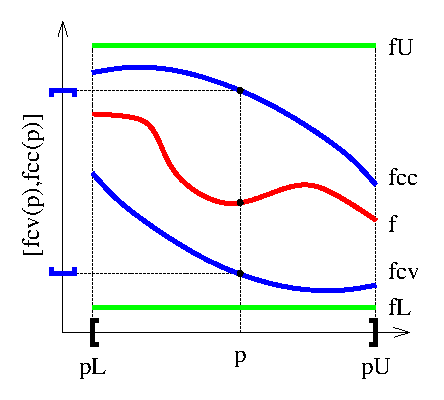
\includegraphics[width=.45\textwidth]{McCormickrelax.eps}

\end{document}
